\section{Tools \& Technologies}
\subsection*{Next.js}
\addcontentsline{toc}{subsection}{Next.js}
The technology stack for the medical prediction website was carefully chosen to
balance performance, scalability, and ease of development. Next.js was selected
for the frontend because it provides a modern React framework with support
for server-side rendering and static site generation, ensuring fast page loads
and a responsive user interface. The complete Next.js application implementation 
is available at \url{https://github.com/ahmed-kaif/hcv-frontend/}.
\subsection*{FastAPI}
\addcontentsline{toc}{subsection}{FastAPI}
FastAPI was chosen for the backend due to
its lightweight design, asynchronous capabilities, and automatic API documentation,
which allows for efficient handling of requests and easy integration with machine learning models.
The backend API is available \url{https://github.com/ahmed-kaif/hcv-ai/}.
\subsection*{SQLite}
\addcontentsline{toc}{subsection}{SQLite}
SQLite serves as the database system because it is lightweight, file-based, and easy to set up without
requiring complex configuration, making it well-suited for rapid development and deployment in small to medium-scale applications.
\subsection*{Scikit-Learn}
\addcontentsline{toc}{subsection}{Scikit-Learn}
Scikit-Learn was used for the machine learning component due to its simplicity,
extensive functionality for classification tasks, and seamless integration with Python,
enabling quick development and deployment of the pretrained HCV prediction model.
\subsection*{Nginx}
\addcontentsline{toc}{subsection}{Nginx}
Nginx was selected as the web server and reverse proxy because of its efficiency
in handling concurrent connections, low resource usage, and strong production reliability.
It enables seamless routing between the Next.js frontend and FastAPI backend, while providing HTTPS support, caching, and static file serving.
Its lightweight design and proven scalability make it an ideal choice for a cost-effective and maintainable deployment.
The following configuration script was used for serving both the frontend app and backend API in local machine and remote VPS server.
\inputminted[fontsize=\footnotesize]{ini}{./codes/nginx.conf}

\subsection*{Docker}
\addcontentsline{toc}{subsection}{Docker}
Docker was chosen to ensure consistent and portable deployments across different environments.
By containerizing the Next.js frontend, FastAPI backend, and supporting services e.g. nginx,
it eliminates dependency conflicts and simplifies setup. Docker also streamlines scaling,
updates, and integration with hosting platforms, making the system easier to manage
and more reliable.
\begin{figure}[htbp]
  \begin{center}
    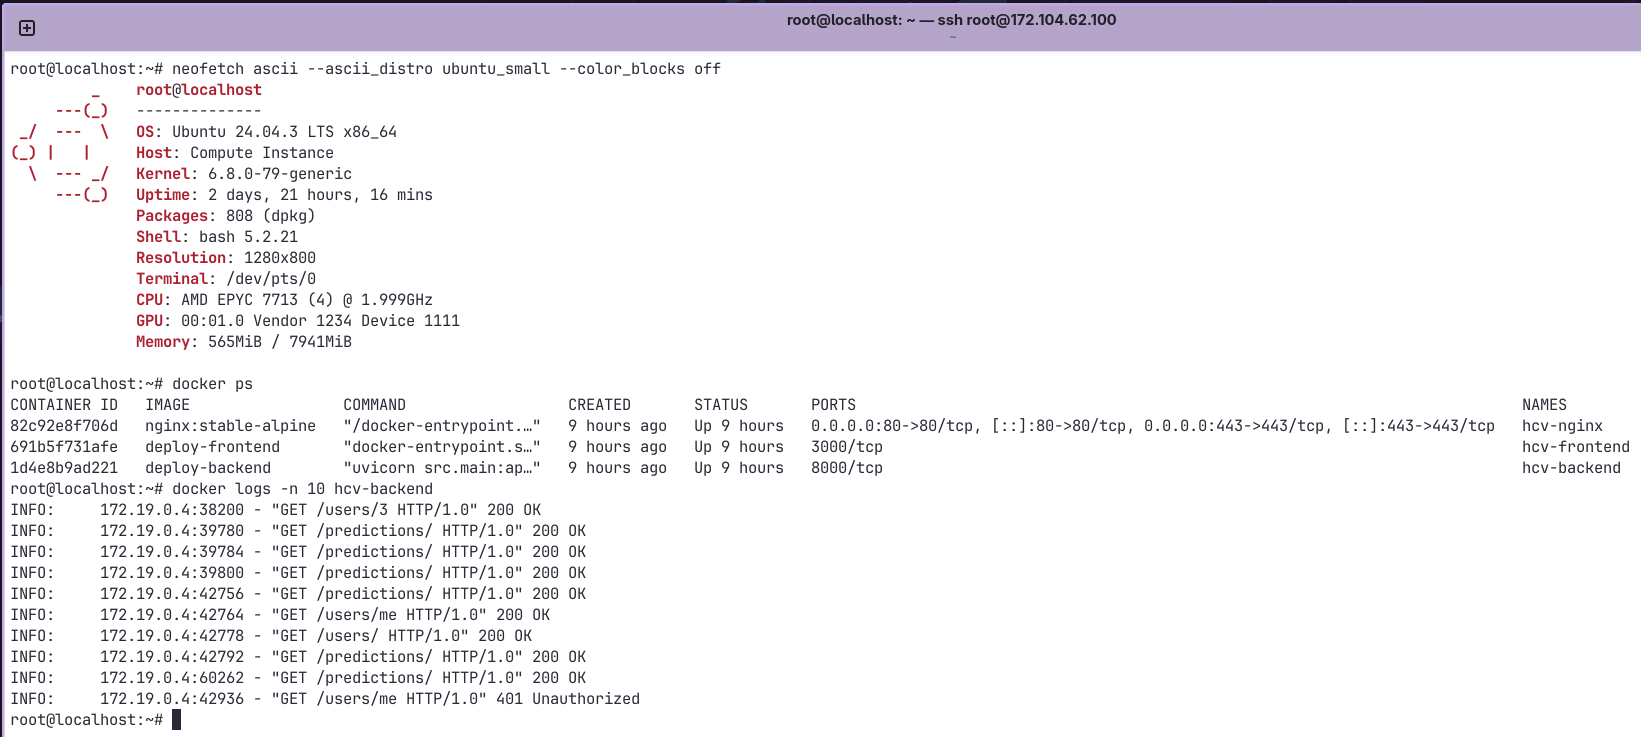
\includegraphics[width=\textwidth]{figures/docker.png}
  \end{center}
  \caption{Docker running on linode ubuntu server vps}\label{fig:docker}
\end{figure}


This combination of technologies ensures that the system is easy to develop, performant,
and maintainable, while also allowing for future migration to more scalable databases if the application grows.
